\chapter[Contrôle postural en VR]{Contrôle postural dans un environnement virtuel}\label{chapII}

La larve de poisson zèbre est intrinsèquement déséquilibrée \cite{bagnall_development_2018}. Son centre de gravité est décalé vers l'avant par rapport à son centre de flottaison, ce qui la fait piquer du nez dans l'axe de tangage. Une larve paralysée se retrouve sur le flanc dans l'axe de roulis. C'est donc par un contrôle permanent qu'elle se maintient à l'horizontale (roulis et tangage). Pour cela, elle utilise à la fois les informations visuelle et vestibulaire pour déclencher des mouvements de queue et de nageoires qui la stabilisent. Ces comportements complexes ont été étudiés en nage libre par David Ehrlich et David Schoppik \cite{ehrlich_control_2017}\cite{ehrlich_balance_2018}\cite{ehrlich_primal_2019}, mais pour comprendre les mécanismes neuronaux à l'œuvre, il est nécessaire de fixer le poisson sous un objectif de microscope. J'ai donc cherché à reproduire ces comportements dans un environnement virtuel en vue d'une étude sous microscope.

\section{Description de la boucle sensorimotrice}

\begin{figure}[b]
    \centering
    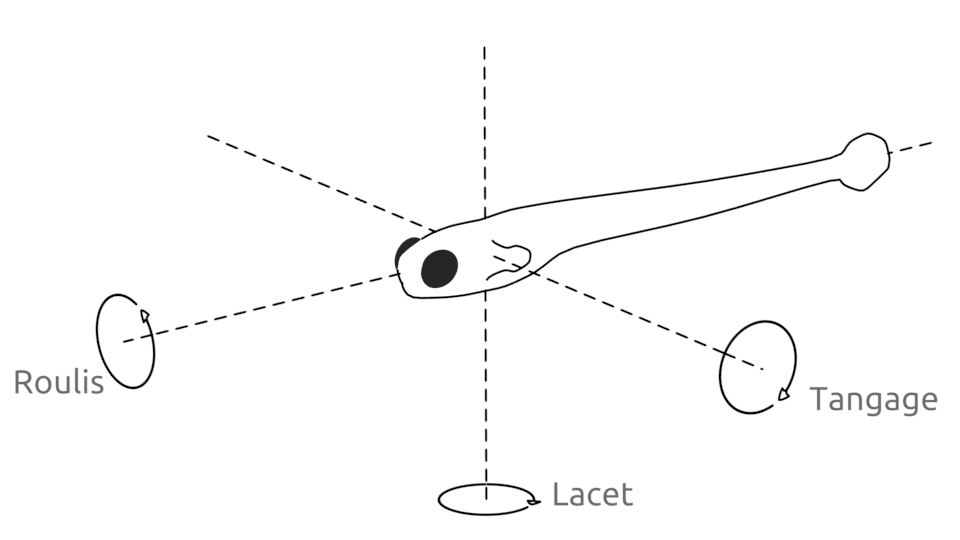
\includegraphics[width=0.8\textwidth]{./files/fish.png}
    \caption{Larve de poisson zèbre dans sa position naturelle. Cette position est hors équilibre, un poisson inactif tourne sur l'axe de roulis et de tangage.
    \label{FIGroulistangage}}
    \end{figure}

La larve de poisson zèbre évolue dans un environnement en trois dimensions. Elle peut se déplacer suivant les trois degrés de liberté en translation et s'orienter suivant les trois degrés de liberté en rotation (Fig. \ref{FIGroulistangage}). Certains comportements comme la thigmotaxie (affection pour les bords) sont liés à sa position dans son environnement, mais dans le cadre du contrôle postural, on s'intéresse surtout à deux degrés de rotation que sont le roulis et le tangage.

\subsection{Roulis}
Dans l'axe de roulis, la larve contrôle son équilibre par des déflexions latérales de la queue. Si elle penche trop à gauche, elle bascule sa queue vers la droite, comme un humain utilisant ses bras pour s'équilibrer. Le contrôle postural en roulis se fait donc par une boucle de rétroaction sensorimotrice continue. L'angle de référence est de 0°, l'organe vestibulaire mesure l'écart à cet angle, et la queue le compense par une déflexion opposée. Ce comportement a été observé par Favre-Bulle \emph{et al} \cite{favre-bulle_optical_2017} en simulant une rotation via une manipulation de l'utricule dans l'oreille interne par des pinces optiques. Cette étude a été réalisée en boucle ouverte, c'est-à-dire sans rétroaction, ce qui fait que la larve ne pouvait pas constater les effets de son mouvement. Une expérience de réalité virtuelle en rétroaction pourrait simuler un déséquilibre proportionnel à l'angle de la queue, ce qui permettrait à la larve d'en corriger l'angle en temps réel.

\subsection{Tangage}

\begin{figure}
    \centering
    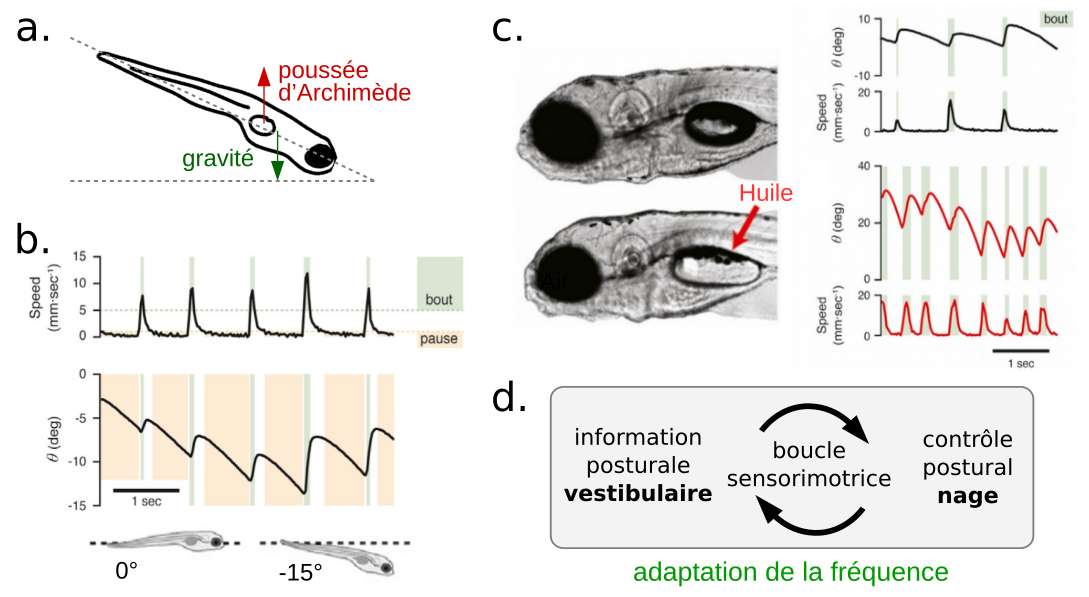
\includegraphics[width=0.9\textwidth]{./files/schoppik_movement-initiation.svg.png}
    \caption{Boucle de rétroaction sensorimotrice et initiation du mouvement lors du contrôle postural en tangage. Adapté de Ehrlich et al \cite{ehrlich_control_2017}
    \\ a. Le centre de gravité et de flottaison de la larve sont décalés, ce qui cause un déséquilibre dans l'axe de tangage.
    \\ b. La larve nage de manière discrète (non continue), à une fréquence de $\sim$1 Hz. Entre deux événements, la larve inactive est entraînée par son déséquilibre, nez vers le bas à une vitesse de $\sim$6°/sec. Lors des événements de nage (pic de vitesse), l'angle est corrigé de $\sim$6°.
    \\ c. En remplaçant l'eau de la vessie natatoire par de l'huile, ce qui augmente le déséquilibre, les auteurs ont constaté une augmentation de la fréquence (diminution de l'IEI, intervalle inter-événement), ce qu'ils attribuent au contrôle de la posture via l'information vestibulaire.
    \\ d. La boucle sensorimotrice discrète responsable du contrôle postural est capable d'une adaptation en fréquence suite à une perturbation de l'équilibre du poisson.
    \label{FIGmovementinitiation}}
    \end{figure}

Dans l'axe de tangage, la situation est plus compliquée. L'angle que fait la larve avec l'horizontale dépend de sa direction de déplacement. Par exemple, une larve se place à un angle positif lorsqu'elle nage vers le haut pour remonter à la surface et un angle négatif quand elle nage vers le bas \cite{ehrlich_primal_2019}. Cet angle constitue une référence autour de laquelle la larve cherche à se stabiliser. Ehrlich et Schoppik ont montré que le contrôle de l'angle se faisait pendant les mouvements de nage \cite{ehrlich_control_2017}. La larve de poisson zèbre nage de manière discrète via des mouvements réguliers à une fréquence d'environ un par seconde en nage libre. Entre deux mouvements, qui peuvent être détectés par des pics de vitesse, elle est soumise à son déséquilibre et bascule vers l'avant à une vitesse angulaire déterminée par sa morphologie. Lors d'un mouvement, en fonction de la force et la position des nageoires, l'angle augmente d'un coup. De plus, les auteurs suggèrent que l'initiation du mouvement est induite par l'angle ressenti. Ils ont augmenté artificiellement le déséquilibre de la larve, conduisant à une chute plus rapide et ont constaté que la larve compensait ce déséquilibre supplémentaire par une augmentation de la fréquence des mouvements de nage (Fig. \ref{FIGmovementinitiation}).
Le contrôle postural en tangage est donc le résultat d'une boucle de rétroaction sensorimotrice discrète. L'angle cible varie entre -15° et +20° environ et dépend de la direction souhaitée par le poisson et d'un certain angle d'attaque \cite{ehrlich_primal_2019}. L'action de contrôle de l'angle implique à la fois la queue et les nageoires et se fait au moment des événements de nage, dont la fréquence peut être ajustée en fonction du déséquilibre.

On voit ici deux boucles sensorimotrices différentes impliquée dans le contrôle postural. Ces boucles de rétroaction ont des caractéristiques différentes en termes de valeur cible et de mécanisme de contrôle. Je décris par la suite une plateforme expérimentale que j'ai mise au point afin d'étudier le contrôle postural en réalité virtuelle.

\section{Étude comportementale du contrôle postural}

\subsection{Plateforme expérimentale}

\begin{figure}[b!]
    \centering
    \includegraphics[width=0.75\textwidth]{./files/schéma_manip.svg.png}
    \caption{Plateforme expérimentale permettant d'étudier le contrôle postural d'une larve de poisson zèbre pendant une boucle de rétroaction. Le système d'imagerie et la cuve sont fixés sur une plateforme rotative, mais pas le projecteur.
    \label{FIGexpplatformbehavior}}
    \end{figure}

Pour reproduire la boucle de rétroaction du contrôle postural, il faut soumettre le poisson à une stimulation vestibulaire, détecter ses mouvements de queue et rétroagir sur son orientation. Avec l'aide de Thomas Panier, j'ai développé une plateforme expérimentale pour répondre à cette problématique (Fig. \ref{FIGexpplatformbehavior}). Elle est constituée d'une cuve où l'on place la larve, d'un système d'imagerie pour suivre les mouvements de queue, d'un projecteur pour projeter un environnement visuel sur les parois de la cuve, d'un moteur pour entraîner la plateforme sur laquelle repose le tout, et d'un ordinateur pour réaliser la boucle de rétroaction. Je décris ci-dessous les différents éléments.

\subsubsection{Stimulation vestibulaire}

Le but de la cuve rotative est de soumettre le poisson à une stimulation vestibulaire contrôlée, et de pouvoir agir rapidement sur la commande (position angulaire, vitesse angulaire). Le moteur que j'ai utilisé pour entraîner la plateforme est le modèle DMAC17 de l'entreprise \href{http://www.midi-ingenierie.com/}{midi-ingéniérie}. Le modèle était assez ancien et ne disposait que d'une interface rudimentaire, j'ai donc dû réimplémenter une commande série pour communiquer avec le microcontrôleur de la commande moteur. Finalement, la communication introduit une latence de quelques dizaines de millisecondes et impose un délai entre deux instructions d'une trentaine de millisecondes. Cela semble cependant suffisant pour garantir une bonne impression de réalité virtuelle, puisque chez l'humain, les effets liés à la latence commencent à se faire sentir à partir de 75 ms \cite{waltemate_impact_2016}. Un problème que j'ai rencontré au début était les mouvements de l'eau dans la cuve. Le poisson y est très sensible via sa ligne latérale postérieure, ce qui faussait les expériences. En perçant un trou en haut de la cuve, j'ai pu la remplir sans laisser d'air et refermer avec un bouchon étanche. Cela a permis de maintenir l'eau de la cuve pratiquement immobile et de contourner ce problème.

\subsubsection{Imagerie et analyse}
Pour détecter de manière fiable les mouvements de queue du poisson, j'ai mis au point un système d'imagerie adapté. Le système doit être léger et compact, afin de limiter le couple lors de la rotation de la plateforme et être insensible aux vibrations. Le poisson est éclairé par une lampe infrarouge à travers un diffuseur et une fenêtre située en haut de la cuve. En bas de la cuve, une autre fenêtre étanche laisse passer la lumière vers un miroir sur lequel pointe une caméra équipée d'un objectif grossissant et d'un filtre infrarouge. L'utilisation de la lumière infrarouge, invisible pour le poisson, permet de conserver la même qualité d'image quel que soit l'environnement visible pour le poisson. Les fenêtres sont les plus petites possible et situées dans l'extrémité du champ de vision du poisson afin de contrôler au mieux son environnement visuel. Le miroir permet de conserver la caméra et l'objectif proche de l'axe de rotation de la plateforme, pour limiter le bras de levier.
L'objectif du système d'imagerie est choisi pour que le poisson soit imagé sur un nombre réduit de pixels de la caméra. Ainsi, le transfert de donnée depuis la caméra vers l'ordinateur et le traitement de l'image sont rapides, ce qui permet de ne pas ralentir la rétroaction. Le traitement de l'image est simple mais fonctionnel. Il consiste à appliquer les fonctions suivantes (Fig. \ref{FIGimageprocessing}) :

\begin{enumerate}[a)] \itemsep0em \setcounter{enumi}{1}
    \item filtre de Sobel (fonction \verb|edge| de Matlab, option \verb|sobel|)
    \item dilatation (fonction \verb|imdilate|)
    \item remplissage (fonction \verb|imfill|)
    \item ouverture (fonction \verb|bwareaopen|)
    \item ellipse équivalente (fonction \verb|regionprops|, option \verb|Orientation|)
\end{enumerate}

Ce qui permet de trouver l'angle du poisson de manière reproductible d'une image sur l'autre, afin de détecter les mouvements de queue.

\begin{figure}
    \centering
    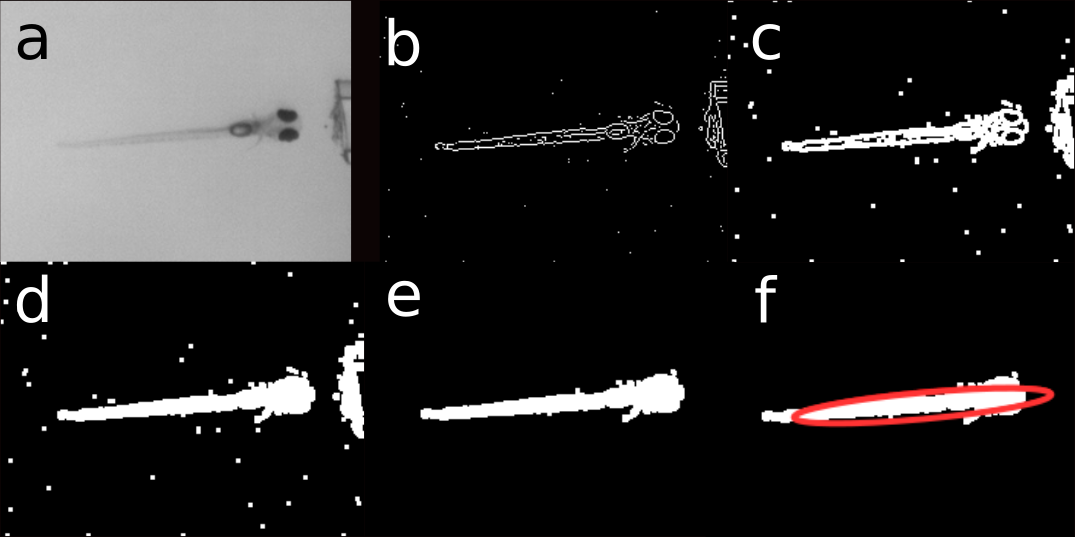
\includegraphics[width=0.8\textwidth]{./files/image_process.png}
    \caption{Traitement d'image en cinq étapes pour obtenir l'angle du poisson. a) image originale sous éclairage infrarouge b) filtre de Sobel c) dilatation morphologique d) remplissage des contours e) ouverture morphologique f) ellipse équivalente via les moments d'ordre deux de l'image
    \label{FIGimageprocessing}}
    \end{figure}

% IGN Volker add figure with tail bend / struggle

\subsubsection{Stimulation visuelle}
Pour avoir un contrôle très souple sur l'environnement visuel du poisson du point de vue des couleurs, de la luminosité, et des formes, la solution idéale est un projecteur. Afin d'obtenir un bon contraste, les parois de la cuve sont coniques et blanches, réalisées dans un cylindre de PVC. Un cache évite d'éclairer directement le poisson pour ne pas perturber son environnement visuel. Les motifs sont réalisés à l'aide de \href{http://psychtoolbox.org/}{psychtoolbox}, une bibliothèque conçue pour l'affichage de stimulations visuelles. Pour conserver une fréquence d'affichage indépendante de la boucle de rétroaction et ainsi garantir un taux constant d'images par seconde d'expérience en expérience, j'ai séparé le processus de la boucle principale, avec laquelle il communique par le protocole TCP/IP.

\subsubsection{Insertion de la larve}

\begin{figure}[b]
    \centering
    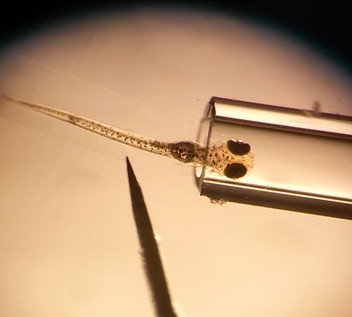
\includegraphics[width=0.5\textwidth]{./files/prepa_larve.jpg}
    \caption{À l'aide d'un scalpel, un boudin d'agar est retiré de la queue d'une larve pour lui permettre de bouger. La larve est retenue par la tête et le corps, l'autre partie du boudin étant tenue par le capillaire en verre.
    \label{FIGagar}}
    \end{figure}

Pour immobiliser la larve de poisson zèbre, il est fréquent de la piéger dans un gel d'agarose à basse température de fusion concentré à 2\% aspiré par un capillaire en verre de diamètre intérieur 0.8 mm. Le capillaire est inséré dans un trou de 1.4 mm (son diamètre extérieur), ce qui le maintient fermement. La larve peut ainsi être placée dans l'une des deux positions suivantes. L'une, sur l'axe de rotation, permet d'étudier la réponse comportementale à une stimulation en roulis, l'autre, perpendiculaire, permet d'étudier la réponse à une stimulation en tangage (Fig. \ref{FIGexpplatformbehavior}). Afin d'observer les mouvements de la queue, je la libère en retirant la partie du boudin d'agarose qui l'entoure (Fig. \ref{FIGagar}). 


\subsection{Protocoles et résultats}

\subsubsection{Test par l'OMR}

\begin{figure}
    \centering
    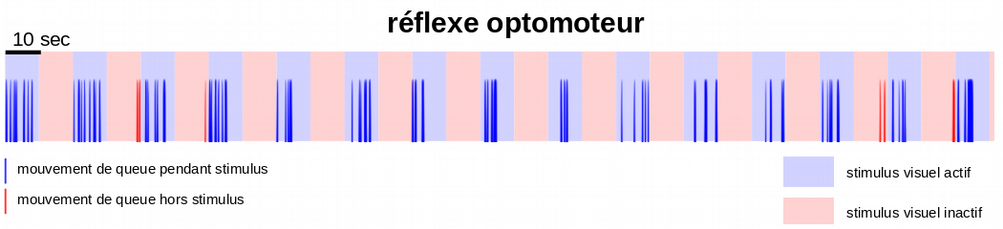
\includegraphics[width=\textwidth]{./files/omr.png}
    \caption{Expérience d'OMR en boucle ouverte. On voit que le poisson nage systématiquement en présence de stimulation visuelle (440 événements sur 150 secondes) et qu'il nage très rarement en absence de stimulation visuelle (22 événements sur 150 secondes).}
    \label{FigOMRopenloop}
    \end{figure}

Après avoir inséré un poisson dans la cuve, je le laisse reposer une à deux minutes pour lui permettre de s'adapter à son nouvel environnement. Je teste ensuite son réflexe optomoteur (OMR). Si le poisson ne réagit pas à cette stimulation visuelle, il est possible que sa vision ou sa motricité ne fonctionne pas, ou que son cerveau ne soit pas dans un état propice à l'étude de son système sensori-moteur. Pour tester l'OMR, je présente une alternance de bandes noires et blanches d'une taille apparente de trente degrés défilant à une vitesse apparente de vingt degrés par seconde, uniquement sur la partie basse de l'environnement visuel. Ce protocole est inspiré par celui présenté par Kris Severi \cite{severi_neural_2014} pour lequel on attend une réponse entre 1 Hz et 5 Hz. J'ai réalisé ce test en boucle ouverte, c'est-à-dire sans rétroaction. Dans ce régime, le poisson présente un phénomène d'habituation si la stimulation dure trop longtemps, j'ai donc alterné des périodes de dix secondes de bandes fixes et dix secondes de bandes mobiles. Dans ces conditions, on observe une réponse à 3 Hz environ lors de la stimulation visuelle, ce qui est cohérent avec les attentes (Fig. \ref{FigOMRopenloop}). Ces expériences sur le réflexe optomoteur montrent que le stimulus visuel projeté est suffisant pour étudier les réponses de la larve à son environnement visuel.

% This is the protocol also in the literature. If I remember correctly this is what Kris used in here paper. It would be good if you add references here

\subsubsection{Rétroaction vestibulaire}\label{subsubretrovestib}

Pour mettre en place la boucle de rétroaction vestibulaire, je me suis inspiré de l'étude en nage libre de Ehrlich \emph{et al} \cite{ehrlich_control_2017}. J'ai choisi une vitesse de chute de -6°/s et une correction angulaire rapide de +10° lors d'un mouvement (en 100 ms environ) (Fig. \ref{FIGvirtualposturalcontrol}). Ainsi, le poisson peut se maintenir à un angle fixe avec un mouvement toutes les 1.6 secondes. Si le poisson est immobile, son angle diminue jusqu'à l'angle limite que j'ai fixé à -60°. Ces expériences ont été réalisées dans le noir ou en éclairage uniforme, pour étudier la perception vestibulaire indépendamment de la perception visuelle.

\begin{figure}
    \centering
    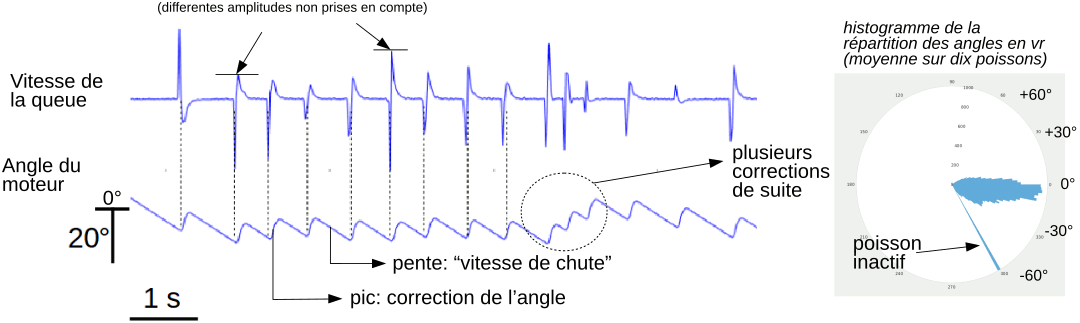
\includegraphics[width=\textwidth]{./files/vestibular_feedback.svg.png}
    \caption{Explication détaillée des étapes du contrôle postural dans une boucle de rétroaction virtuelle. Le poisson est soumis à un stimulus vestibulaire constant (pente constante) en l'absence de comportement. Lors d'un mouvement de nage, une rétroaction sur l'angle de la plateforme simule une correction d'angle du poisson.
    \label{FIGvirtualposturalcontrol}}
    \end{figure}

    
\begin{figure}
    \centering
    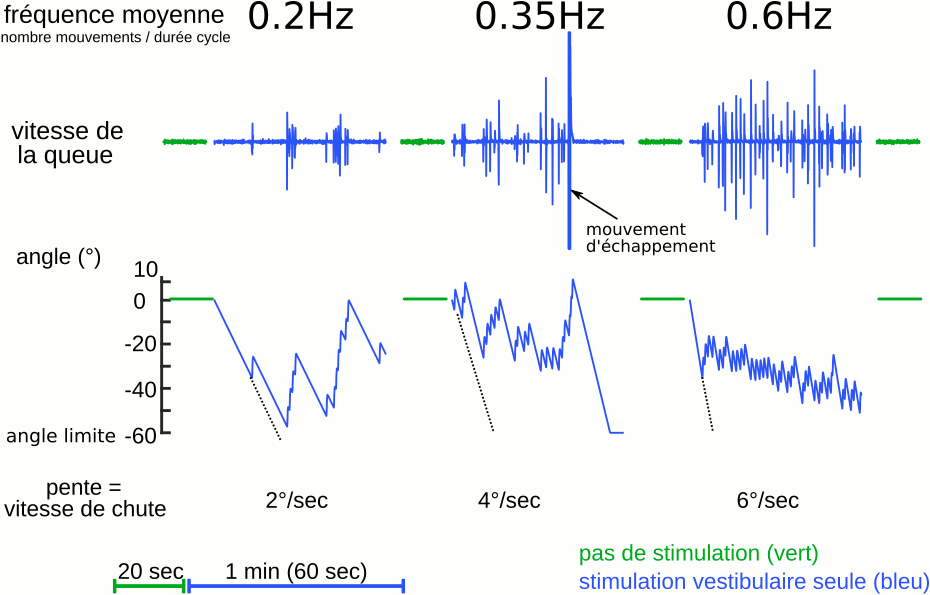
\includegraphics[width=\textwidth]{./files/variation-vitesse.svg.png}
    \caption{
    Réponse d'une larve à une variation de la vitesse de chute. Trois cycles de une minute de stimulation vestibulaire sont séparés de pause de dix secondes. Le poisson se maintient autour d'un angle de -20° quelle que soit la vitesse de chute imposée, en adaptant la fréquence de ses mouvements.
    \\La fréquence moyenne du deuxième cycle est légèrement inférieure à sa valeur attendue (0.35 Hz au lieu de 0.4 Hz). Cela est dû au fait que, suite à un mouvement d'échappement, le poisson est totalement inactif à la fin du cycle et stationne à -60°. Si l'on calcule la fréquence en ignorant les dix dernières secondes, la fréquence moyenne est bien de 0.4 Hz.
    \label{FIGvariationvitesse}}
    \end{figure}


Les paramètres de la boucle sont la vitesse de chute et l'angle de correction lors du mouvement. Pour répondre à une modification de ces paramètres, le poisson doit adapter la fréquence de ses mouvements, car l'amplitude n'est pas prise en compte. Ainsi, à correction angulaire fixe, si la vitesse de chute augmente, comme dans l'expérience de la vessie natatoire remplie d'huile, le poisson doit augmenter la fréquence de ses mouvements. Au contraire, à vitesse de chute fixe, si la correction angulaire augmente, le poisson doit baisser la fréquence de ses mouvements. C'est effectivement ce que l'on constate dans les expériences, où une vitesse de chute de -2°/s, -4°/s et -6°/s avec une correction angulaire de 10° entraînent respectivement chez la larve une fréquence de mouvement de 0.2 Hz, 0.4 Hz, et 0.6 Hz en moyenne (figure \ref{FIGvariationvitesse}).

% ok GeorgesComment
% il faut discuter du nombre de poissons testés, statistiques/poisson, etc...

La principale difficulté de ces expériences est le fait que le poisson peut devenir inactif et stationner à l'angle minimal autorisé par le système (-60°). C'est pour cette raison que la durée choisie pour les cycles est relativement courte (60 secondes). À la fin d'un cycle, le poisson est ramené à l'angle de référence (0°). Cela évite que le poisson reste trop longtemps inactif, état dans lequel il est impossible d'étudier le contrôle postural. Pour obtenir des fréquences représentatives, il faut donc les calculer uniquement sur les périodes d'activité.

On observe ce même comportement sur des larves dans une boîte de pétri : de temps en temps elles cessent toute activité et reposent sur le fond de la boîte. La boucle de rétroaction du contrôle postural est alors en pause. Dans le cas d'une larve prisonnière d'un boudin d'agarose, les périodes d'inactivité font souvent suite à un mouvement d'échappement, pendant lequel la larve tente de s'échapper en déclenchant des mouvements de très grande amplitude.

\subsubsection{Protocole multimodal}

\begin{figure}
    \centering
    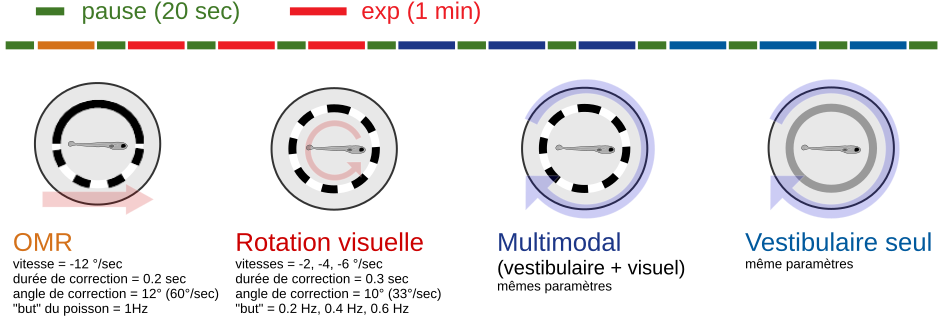
\includegraphics[width=0.95\textwidth]{./files/protocole_multimodal.svg.png}
    \caption{
    Protocole multimodal faisant intervenir à la fois une stimulation vestibulaire et une stimulation visuelle. Les différentes étapes du protocole sont schématisées par une vue de côté de la larve dans la cuve exposée à différents stimuli (visuel en rouge, vestibulaire en bleu). Les barres colorées en dessous représentent la chronologie des étapes du protocole : des cycles d'une minute (OMR, visuel, multimodal, vestibulaire) sont séparés par des pauses de vingt secondes.
    On présente la réponse de trois poissons différents (a, b, c.) sous la même forme qu'en figure \ref{FIGvariationvitesse} (en haut la vitesse de la queue et en bas l'angle de la plateforme). Dans tous les cas, la réponse optomotrice fonctionne, mais on voit des différences au niveau des autres stimuli. Le poisson (a.) répond bien à la stimulation visuelle, mais quasiment pas à la stimulation vestibulaire, le poisson (b.), au contraire, ne répond pas à la stimulation visuelle (bien qu'il réponde à l'OMR), mais répond à la stimulation vestibulaire pure. Le poisson (c.) ne répond ni à la stimulation visuelle pure, ni à la stimulation visuelle pure, mais répond comme les deux autres pendant le cycle multimodal.
    \label{FIGprotocolmulti}}
    \end{figure} 

L'intérêt de l'environnement virtuel est qu'il est possible de contrôler à la fois la stimulation vestibulaire et la stimulation visuelle. Après avoir étudié le contrôle postural dans le noir, j'y ai ajouté une composante visuelle. L'objectif est de comparer la réponse en cas de stimulation multimodale par rapport aux réponses en présence des deux stimuli séparément.

Le protocole (illustré en Fig. \ref{FIGprotocolmulti}) comporte les étapes suivantes. 

\begin{enumerate}
    \item Il commence par un cycle d'OMR avec rétroaction, qui permet d'évaluer le niveau d'activité du poisson. S'il ne répond pas à cette stimulation, l'expérience est interrompue pour passer au poisson suivant, ce qui permet de gagner un quart d'heure en évitant de collecter des données sur une larve immobile.
    \item Ensuite vient une phase de stimulation purement visuelle avec rotation de l'ensemble de l'environnement, tout autour du poisson. Pendant cette phase, l'information visuelle indique au poisson qu'il tourne, ce qui est en conflit avec l'information vestibulaire. La partie inférieure du champ visuel est similaire à une stimulation d'OMR, mais la partie supérieure diffère.
    \item Tout en conservant le motif de la phase visuelle en position fixe dans le référentiel du laboratoire, la cuve tourne ensuite avec le poisson pour stimuler le système vestibulaire, utile au contrôle postural. Pendant cette phase, les deux modalités sensorielles sont cohérentes. Elles indiquent toutes les deux au poisson qu'il est en train de tourner.
    \item Enfin, le motif est remplacé par un éclairage uniforme d'intensité moyenne identique. Cela permet de conserver une luminosité ambiante dans la cuve identique au cycle précédent. Cette phase est celle exposée précédemment (section \ref{subsubretrovestib}).
\end{enumerate}

Chaque phase est séparée en trois sous-phases, avec trois vitesses de stimulus différentes (2, 4, et 6 degrés par seconde), pour étudier l'adaptation aux conditions virtuelles.

% IGN discuter de la distinction entre OMR et rotation visuelle

Sur un total de 113 larves préparées, 24 se sont échappées ou sont mortes avant l'expérience (reste 89), j'ai appliqué le protocole décrit ci-dessus et 53 larves ne présentaient aucune réponse optomotrice, ou seulement des tentatives d'échappement (reste 36). Sur ces 36 larves restantes, qui présentaient donc toutes une réponse optomotrice, 24 ont montré une réponse quasi nulle lors des autres étapes du protocole et ont donc été retirée du compte (reste 12). Les 12 larves restantes ont eu des réponses différentes au protocole. Certaines (3) répondaient principalement au stimulus visuel seul ou bimodal (Fig. \ref{FIGprotocolmulti} a.), certaines (5) répondaient principalement au stimulus vestibulaire seul ou bimodal (Fig. \ref{FIGprotocolmulti} b.), certaines (4) surtout au stimulus bimodal (Fig. \ref{FIGprotocolmulti} c.).

\begin{figure}
    \centering
    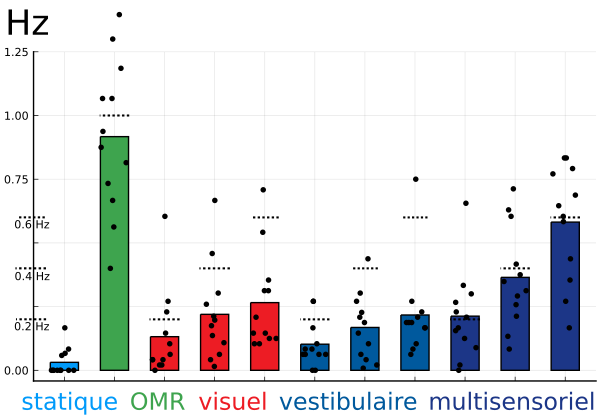
\includegraphics[width=\textwidth]{./files/stats3.svg.png}
    \caption{
    Fréquence moyenne des mouvements de queue de douze poissons en réponse au protocole (Fig. \ref{FIGprotocolmulti}). Chaque point représente la valeur pour un poisson moyennée sur une à quatre répétitions du protocole, la barre colorée représente la valeur moyenne. Les valeurs "cible" précisées dans le protocole (0.2 Hz, 0.4 Hz, 0.6 Hz) sont représentées par des barres en pointillé. Pour chaque cycle, on observe une adaptation du poisson à la force du stimulus. Le poisson est capable d'adapter sa fréquence de nage pour se stabiliser par rapport à une information visuelle ou vestibulaire. Pour chaque vitesse de stimulus, on observe une réponse moyenne différente en fonction du type de stimulus. Alors que le stimulus vestibulaire et visuel pur sont d'efficacité comparable, la présence simultanée des deux modalités sensorielles entraîne globalement une meilleure réponse chez les larves.
    \label{FIGstatsmultimodal}}
    \end{figure}

\subsubsection{Interprétation}

Il semble donc qu'en fonction des poissons l'importance relative des différentes modalités sensorielles dans le contrôle postural soit variable. Pour certains poissons, cependant, la présence simultanée des deux modalités sensorielles semble nécessaire au contrôle postural. Ces données peuvent être interprétées en termes de fréquence moyenne calculée comme le rapport entre la quantité de mouvements de nage et la durée du cycle. Cette métrique inclut les périodes d'inactivité qui suivent un mouvement d'échappement, ce qui fausse légèrement la valeur, comme montré en figure \ref{FIGvariationvitesse}. Les résultats sont présentés en figure \ref{FIGstatsmultimodal} et l'on observe deux phénomènes :

\begin{enumerate}
    \item Une larve est capable de moduler son activité en fonction de la force du stimulus.
    \item Une larve a une réponse accrue en présence de deux stimuli cohérents.
\end{enumerate}

Ces résultats montrent qu'un réflexe \emph{a priori} vestibulaire comme le contrôle postural est en réalité altéré par d'autres modalités sensorielles comme le système visuel. On peut supposer que la sensation tactile, qui permet au poisson de sentir les écoulements de fluide, joue également un rôle (non testé). 

Le renforcement multisensoriel peut être interprété ainsi : pendant les phases unimodales visuelles, les sensations visuelle et vestibulaire sont en conflit, ce qui peut réduire et même supprimer la réponse motrice, la force de cet effet variant d'un poisson à l'autre. Dans les phases unimodales vestibulaires, le poisson ne reçoit aucune information visuelle sur sa position et la réponse comportementale peut être affaiblie par un manque de fiabilité de l'information vestibulaire. Au contraire, pendant les phases de stimulus multimodal cohérent, on remarque une réponse comportementale forte, augmentée par l'intégration multisensorielle.

% Volker suggestion
% During the unimodal visual phases the visual and vestibular sensations are in conflict reducing or suppressing the motor response. The strength of this effect varies between fish. In the unimodal vestibular case where the fish does not receive and visual information about its body rotation the behavioral response might be weak due to the unrelieability of the vestibular stimulus. However, in the coherent multimodal case we see a strong multisensory enhanced behaviorial response 

\subsection{Ouverture}

Comme montré, ce système permet de reproduire la boucle de rétroaction sensorimotrice du contrôle postural dans un environnement virtuel. Cependant, une limitation importante réside dans les longues périodes d'inactivité qui suivent souvent les mouvements d'échappement de la larve. 
Ces périodes réduisent considérablement la quantité de données exploitables. Le poisson est en effet quasiment inactif dans environ neuf expériences sur dix, ce qui explique mon échantillon statistique faible.
Ces comportements d'abandon pourraient être expliqués par un article de Mu \emph{et al} \cite{mu_glia_2019}. Celui-ci décrit comment, suite à une action infructueuse de la larve, des cellules gliales accumulent l'information jusqu'à inhiber le comportement perçu comme inutile.
Dans le cas d'une larve immobilisée dans un gel d'agarose, si les mouvements de queue de grande amplitude qui caractérisent l'échappement se soldent par une réussite, la larve s'échappe dans le réservoir, mettant fin à l'expérience, et si, au contraire, ils se soldent par un échec, la larve finit par abandonner toute réponse comportementale, réduisant à zéro le nombre d'événements à analyser.

Une piste d'évolution importante serait donc de limiter ces comportements d'échappement. Cela permettrait de réaliser des expériences plus longues et plus complexes afin de mettre à l'épreuve ces observations préliminaires et d'observer d'autres phénomènes.
Dans les comportements observés, il semblerait que certains poissons répondent mieux à la stimulation visuelle et d'autres mieux à la stimulation vestibulaire. Des expériences plus longues avec plus de cycles permettraient de mettre en évidence ces spécificités individuelles des larves. Par exemple, en figure \ref{FIGprotocolmulti}, l'expérience a été reproduite cinq fois d'affilée sur le poisson (c.) : malgré une réponse systématique à l'OMR, le poisson montre peu de réponse pour un stimulus visuel seul, il répond fortement en présence d'un stimulus vestibulaire accompagné d'un stimulus visuel, mais pas en présence d'un stimulus vestibulaire seul. Ce poisson semble présenter un renforcement multisensoriel robuste.

Des expériences plus longues permettraient aussi de s'intéresser à la question de l'angle cible. Dans la stabilisation en roulis, l'angle cible est fixé à 0°, mais dans la stabilisation en tangage, il peut varier entre des valeurs comprises entre -15° et +20°. Ces valeurs observées en nage libre par Ehrlich et Schoppik \cite{ehrlich_primal_2019} sont associées à des trajectoires allant de -40° à +80° avec une relation affine liée à l'utilisation des nageoires pectorales. La reconstruction de trajectoires virtuelles paraît hors de portée, mais l'on pourrait observer l'évolution de l'angle cible. Reproduit sous microscope, ce comportement permettrait d'identifier les circuits responsables du choix de cet angle, peut être sous forme de copie efférente.

Si l'immobilisation de la larve est responsable de ces comportements d'échappement, on pourrait modifier la manière dont la larve est immobilisée par exemple en changeant la méthode de préparation du gel d'agarose. Les paramètres de rétroaction pourraient également être en cause, et leur ajustement pourrait augmenter l'immersion de la larve dans son environnement virtuel. Sans de telles améliorations, l'expérience serait difficile à reproduire sous microscope, car l'imagerie vient avec un nouveau lot de contraintes, comme nous allons le voir dans les parties suivantes.

% escape/startle/struggle
% IGN lire et intégrer ces papiers
% - Glia Accumulate Evidence that Actions Are Futile and Suppress Unsuccessful Behavior
% - Escape Behavior Elicited by Single, Channelrhodopsin-2-Evoked Spikes in Zebrafish Somatosensory Neurons
% - Imaging the Functional Organization of Zebrafish Hindbrain Segments during Escape Behaviors
% - Evidence for a Widespread Brain Stem Escape Network in Larval Zebrafish
% - Imaging escape and avoidance behavior in zebrafish larvae

% IGN Volker Perspective and interpretation of the results is still to develop.
